\algblockdefx{RepeatUntil}{EndRepeatUntil}{\textbf{repeat until}}{}
\algnotext{EndRepeatUntil}

\section{Semi-Analytical Primal Solver}
\label{sec:sap_solver}

The Semi-Analytical Primal Solver (SAP) is an iterative algorithm inspired
by Newton's method for solving the unconstrained  formulation (\ref{eq:primal_unconstrained}). Exploiting differentiability of the objective
$\ell_p(\mf{v})$, it selects a search direction $\Delta\mf{v}$ at each iteration using the
formula
\[
  \Delta\mf{v} =  \mf{H}(\mf{v})^{-1} \nabla \ell_p(\mf{v}),
\]
where $\mf{H}(\mf{v})$ is a positive-definite weighting
matrix. It then descends the cost function along this direction
using line-search.  When $\nabla \ell_p(\mf{v})$ is differentiable,
$\mf{H}(\mf{v})$ returns the Hessian matrix $\nabla^2 \ell_p(\mf{v})$.
Otherwise, $\mf{H}(\mf{v})$ is evaluated by extending
analytical expressions for $\nabla^2 \ell_p$ to points
of non-differentiability, see Appendix \ref{app:gradients_derivation}.  As we show \RedHighlight{TODO: reference to Frank's proofs}, SAP 
globally convergences at least at a linear-rate.
Further, SAP exhibits quadratic convergence when
$\nabla^2 \ell_p$ exists in a neighborhood of the
optimal $\mf{v}$.
In practice, we initialize SAP at the previous time-step velocity $\mf{v}_0$.
The stopping criteria is discussed below in Section
\ref{sec:stopping_criteria}.

\begin{algorithm}[H]
  \caption{The Semi-Analytical Primal Solver (SAP)}	
	\label{alg:sap}
	\begin{algorithmic}[1]
		\State Initialize $\mf{v}^0 \gets \mf{v}_0$
		\RepeatUntil $~\Vert\tilde{\nabla}\ell_p\Vert < \varepsilon_a + \varepsilon_r\max(\Vert\tilde{\mf{p}}\Vert,\Vert\tilde{\mf{j}_c}\Vert)$, Eq. \eqref{eq:stopping_criteria}
			\State $\Delta\mf{v}^{m} = -\mf{H}^{-1}(\mf{v}^m)\nabla_\mf{v}\ell_p(\mf{v}^m)$ \label{op:Newton_iteration}
			\State $\displaystyle \alpha^m = \argmin_{t\in\mathbb{R}^{++}} \ell_p(\mf{v}^m + t \Delta\mf{v}^{m})$
			\State $\displaystyle \mf{v}^{m+1} = \vf{v}^m + \alpha^{m}\Delta\mf{v}^{m}$
		\EndRepeatUntil
		\State\Return $\{\mf{v}$, $\bgamma=P_\mathcal{F}(\vf{y}(\mf{v}))\}$
	\end{algorithmic}
\end{algorithm}

The line-search algorithm is critical to the success of SAP
given that $\nabla \ell_p(\mf{v})$ can rapidly change during 
contact-mode transitions.  We explore two line-search
algorithms: an approximate backtracking line-search with Armijo's stopping
criteria and an exact (to machine epsilon) line-search. We show how a careful
pre-computation of commonly occurring terms enables the exact line-search step
at a small fraction of the total cost. Though both line-search approaches
guarantee the convergence of SAP \RedHighlight{ref to Frank's proof}, we find
that the exact line-search can lead to a performance improvement between 15\% to
35\%. In the next subsections, we describe each component of the solver in
detail.

\subsection{Gradients}
\label{sec:gradients}

We provide a detailed derivation of the gradients in Appendix
\ref{app:gradients_derivation}. Here we summarize the main results required for
implementation. The gradient of the
primal cost $\ell_p$ is
\begin{equation*}
	\nabla_\mf{v}\ell_p(\mf{v}) = \mf{A}(\mf{v}-\mf{v}^*) + \nabla_\mf{v}\ell_R,
\end{equation*}
where we define the regularizer cost as $\ell_R(\mf{v})=\frac{1}{2}\Vert
P_\mathcal{F}(\mf{y}(\mf{v}))\Vert_R^2$. This gradient can be computed analytically as
\begin{equation}
	\nabla_\mf{v}\ell_p(\mf{v}) = \mf{A}(\mf{v}-\mf{v}^*) - \mf{J}^T\bgamma(\mf{v})
	\label{eq:primal_gradient}
\end{equation}
where $\bgamma(\mf{v})=P_\mathcal{F}(\vf{y}(\mf{v}))$ is defined by the analytical inverse
dynamics in Eq. \eqref{eq:analytical_y_projection}. 
The map $P_\mathcal{F}(\mf{y}(\mf{v}))$ is differentiable
when $\mf{y}$ is not on the boundary of $\mathcal{F}$.
At these points, we obtain the Hessian of $\nabla_\mf{v}^2\ell_R$  by differentiating $\bgamma(\mf{v})$ and extend the analytical expressions to points of non-differentiability. The result is
\begin{eqnarray}
	\nabla_\mf{v}^2\ell_R(\mf{v}) &=& \mf{J}^T\mf{G}\,\mf{J}\nonumber\\
	\mf{G} &=&-\nabla_{\mf{v}_c}\bgamma = \nabla_\mf{y}\bgamma \mf{R}^{-1}
	\label{eq:ellR_hessian}
\end{eqnarray}
where $\nabla_{\mf{v}_c}\!\bgamma$ is a block diagonal matrix where each
diagonal block is the $3\times 3$ matrix $\nabla_{\mf{v}_{c,i}}\!\bgamma_i$
for the $i\text{-th}$ contact. As shown in Appendix
\ref{app:gradients_derivation}, $\nabla_{\mf{v}_c}\bgamma\succeq 0$ and thus
$\nabla_\mf{v}^2\ell_R(\mf{v})\succeq 0$.

In total, when $\nabla_\mf{v}^2\ell_R$ is well-defined,
we evaluate $\mf{H}$ via: 
\begin{equation}
	\mf{H} = \mf{A} + \mf{J}^T\mf{G}\,\mf{J}
	\label{eq:ell_hessian}
\end{equation}
which, since $\mf{A}\succ 0$, is strictly positive definite. Notice
that to compute the required gradient and Hessian, we need analytical expressions
for the projection $P_\mathcal{F}(\vf{y})$ and its gradient
$\nabla_\mf{y}P_\mathcal{F}(\vf{y})$. They are provided in Appendices
\ref{app:analytical_inverse_dynamics_derivations} and
\ref{app:gradients_derivation} respectively.

\subsection{Line Search}

At the $m\text{-th}$ Newton iteration, backtracking line-search starts with a
maximum step length of $\alpha_\text{Max}$ and progressively decreases it
by a factor $\rho \in (0, 1)$ as $\alpha\gets\rho\alpha$ until Armijo's
criteria \cite[\S 3.1]{bib:nocedal2006numerical} is satisfied. We write Armijo's
criteria as $~\ell_p(\mf{v}^m + \alpha \Delta\mf{v}^{m}) < \ell_p(\mf{v}^m) +
c\,\alpha\,d\ell_p/d\alpha(\mf{v}^m)$. Typical parameters we use are
$\rho=0.8$, $c=10^{-4}$ and $\alpha_\text{Max}=1.5$.

Since the cost $\ell_p(\mf{v})$ is strongly convex and differentiable with
Lipschitz continuous gradients, see Lemma \RedHighlight{reference to Frank's
proof}, its restriction to a line $\ell(\alpha)$ inherits the following
properties
\begin{enumerate}
	\item $\ell_p(\alpha)$ is strongly convex, i.e. there is a unique minimum.
	\item $\ell_p(\alpha)$ is a once, but not twice, differentiable. 
      \item With the prescribed regularization for friction 
        and stiff compliance (Section~\ref{sec:understanding_model_parameters}),
	gradients of $\ell_p(\alpha)$ can change rapidly, even within 
        the same contact mode.
\end{enumerate}

This leads us to choose a one-dimensional strategy that is robust under these
conditions. We find the method \verb;rtsafe; in \cite[\S
9.4]{bib:numerical_recipes} to work the best. \verb;rtsafe; is a one-dimensional
root finder that uses the Newton-Raphson method and switches to bisection
whenever Newton's method leads to an iterate outside a search bracket or
whenever its convergence is slow. Using analytical first and second derivatives
(analytically extended to points of non-differentiability),
our line search simply reduces to finding the unique root of $d\ell/d\alpha$
using the \verb;rtsafe; algorithm. The high performance of this method allows us 
to iterate $\alpha$ to machine precision at a negligible impact on the
computational cost. In practice, this is our preferred algorithm since it allows
us to use very low regularization parameters without having to tune tolerances
in the line search. Moreover, we observe 15\%-35\% performance improvement when
compared to the backtracking line-search.

\subsection{Efficient Analytical Derivatives For Line Search}

The algorithm \verb;rtsafe; requires the first and second directional
derivatives of $\ell_p$, while the
backtracking method only requires the first derivative to verify Armijo's
stopping criteria. We show how to compute these derivatives efficiently in
$\mathcal{O}(n)$ operations. To simplify exposition, we assume
that $\nabla^2 \ell_p(\mf{v})$ exists so that the second-derivative is well-defined.

Defining $\ell(\alpha) = \ell_p(\mf{v}+\alpha\Delta\mf{v})$, we can compute first
and second derivatives with respect to $\alpha$ using the gradient and Hessian
\begin{eqnarray}
	\frac{d\ell}{d\alpha}&=&\Delta\mf{v}^T\nabla_\mf{v}\ell(\alpha)\nonumber\\
	\frac{d^2\ell}{d\alpha^2}&=&\Delta\mf{v}^T\nabla_\mf{v}^2\ell(\alpha)\Delta\mf{v}\nonumber
\end{eqnarray}

These derivatives are expensive to compute for general non-linear functions, and
most line search variations in practice are approximations that avoid their
computation altogether. For $\ell_p$, we  show they can be
computed efficiently.

Using the gradients from Section \ref{sec:gradients}, we can write
\begin{eqnarray}
	\frac{d\ell_M}{d\alpha}(\alpha)&=&\Delta\mf{v}^T\mf{A}(\mf{v}(\alpha)-\mf{v}^*)\\
	\frac{d\ell_R}{d\alpha}(\alpha)&=&-\Delta\mf{v}^T\mf{J}^T\bgamma.
\end{eqnarray}
These are computed efficiently by first calculating the change in velocity
$\Delta\mf{v}_c:=\mf{J}\Delta\mf{v}$ and change of momentum $\Delta\mf{p} :=
\mf{A}\Delta\mf{v}$. The calculation is then completed via 
\begin{eqnarray}
	\frac{d\ell_M}{d\alpha}(\alpha)&=&\Delta\mf{p}^T(\mf{v}(\alpha)-\mf{v}^*)\\
	\frac{d\ell_R}{d\alpha}(\alpha)&=&-\Delta\mf{v}_c^T\bgamma(\alpha)
\end{eqnarray}
which only require dot products that can be computed in $\mathcal{O}(n_v)$ and
$\mathcal{O}(n_c)$ respectively.

Using the same definitions, we can write simple expressions for the second
derivatives as well
\begin{eqnarray}
	\frac{d^2\ell_M}{d\alpha^2}(\alpha)&=&\Delta\mf{v}^T\mf{A}\Delta\mf{v}=\Delta\mf{v}^T\Delta\mf{p}\\
	\frac{d^2\ell_R}{d\alpha^2}(\alpha)&=&-\Delta\mf{v}_c^T
	\nabla_{\mf{v}_c}\bgamma\Delta\mf{v}_c.
\end{eqnarray}
Notice that $\frac{d^2\ell_M}{d\alpha^2}$ is independent of $\alpha$ and
can be precomputed before the line search, and
$\frac{d^2\ell_R}{d\alpha^2}$ only involves $\mathcal{O}(n_c)$ operations given
the block diagonal structure of $\nabla_{\mf{v}_c}\bgamma$.

\subsection{Problem Sparsity}
\label{sec:problem_sparsity}




Each iteration of SAP requires the solution of the linear system
$\mf{H}(\mf{v}^m)\Delta\mf{v}^{m} = -\nabla_\mf{v}\ell_p(\mf{v}^m)$.
The matrix $\mf{H}(\mf{v}^m)$ inherits a block sparse structure from
the specific contact configuration of the problem. 
We exploit this structure using a supernodal Cholesky factorization \cite[\S
9]{bib:davis2016survey}. Implementing this factorization requires construction
of a \emph{junction tree}.  For this we apply the algorithm in
\cite{bib:smail2017junction}, using cliques of $\mf{H}$ as input. We
use the implementation from the Conex solver \cite{bib:permenter2020}.

The block sparsity of $\mf{H}$  is best described with an example. We organize
our multibody systems as a collection of articulated \emph{tree structures}, or
a \emph{forest}. Consider the system in Fig. \ref{fig:sparsity_example}.
\begin{figure}[!h]
	\centering
	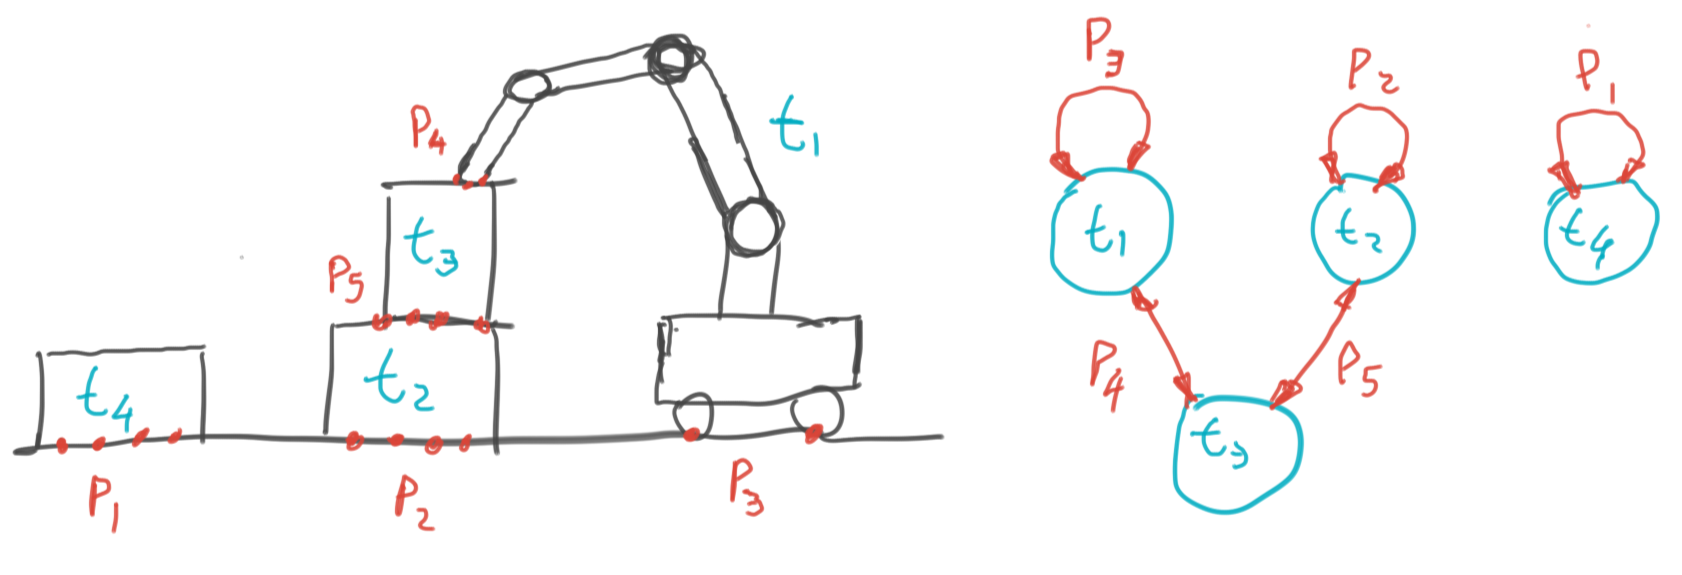
\includegraphics[width=0.7\columnwidth]{figures/sparsity_example.png}
	\caption{\label{fig:sparsity_example} 
	An example of a sparsity pattern commonly encountered in the
	simulation of robotic mechanical systems. The graph on the right puts
	\textit{trees} as nodes and contact \textit{patches} as edges. Notice how
	this graph exactly describes the sparsity pattern of the matrix
	$\mf{J}^T\mf{G}\mf{J}$ in Fig. \ref{fig:JTGJ_schematic}.}
\end{figure}
In this example, a robot arm mounted on a mobile base constitutes its own tree,
here labeled $t_1$. The number of degrees of freedom of the $t\text{-th}$ tree
will be denoted with $n_t$. A free body is the common case of a tree with
$n_t=6$. In general, the mass matrix will have a
block diagonal structure where the $t\text{-th}$ diagonal block corresponds to
the mass matrix of the $t\text{-th}$ tree. For the example in Fig.
(\ref{fig:sparsity_example}), the mass matrix looks like\\\\\\
\begin{equation}
	\mf{M}=\quad
	\begin{bmatrix}
		\tikzmark{M_topleft}
		\diagentry{\mf{M}_{\cc{11}}}&&&\tikzmark{M_topright}\\
		&\diagentry{\mf{M}_{\cc{22}}}\\
		&&\diagentry{\mf{M}_{\cc{33}}}\\		
		\tikzmark{M_bottomleft}&&&\diagentry{\mf{M}_{\cc{44}}}
	\end{bmatrix}
% Draw lil arrows on top and to the left.
\tikz[overlay,remember picture] {
	\draw[->,thick,color=cyan]
  ([yshift=3ex]M_topleft) -- ([yshift=3ex]M_topright) node[midway,above]
  {\scriptsize $t$}; 
  \draw[->,thick,color=cyan]
  ([yshift=1.5ex,xshift=-2ex]M_topleft) -- ([xshift=-4ex]M_bottomleft)
  node[near end,left] {\scriptsize $t$};}	
\end{equation}
\RedHighlight{Make this equation a Figure instead.}

We define as \textit{patches} a collection of contact pairs between two
trees. We label in red all contact patches in Fig. (\ref{fig:sparsity_example}).
Each contact pair corresponds to a single cone constraint in our
formulation. The set of constraint indexes that belong to patch $p$ is
denoted with $\mathcal{I}_p$ of size (cardinality) $|\mathcal{I}_p| = r_p$.

Notice that our definition of \textit{patches} is used to describe sparsity and
has nothing to do with the actual geometrical topology of the contact surface
between two trees. That is, the \textit{patches} could in
general correspond to either a single connected surface or a complex contact area
formed by a set of disconnected surfaces. Figure (\ref{fig:sparsity_example})
labels trees and patches and shows the corresponding graph where the nodes are
the trees and the edges are the contact patches.

Recall from Eq. (\ref{eq:ellR_hessian}) that $\mf{G} =
-\nabla_{\mf{v}_c}\bgamma$ is a block diagonal matrix, with $\vf{G}_i =
\nabla_{\vf{v}_{c,i}}\bgamma_i \in \mathbb{R}^{3\times 3}$ at the $i\text{-th}$
diagonal block. We can also write this as $\mf{G} = \text{diag}(\mf{G}_p)$ if we
group contact pairs by patches to define $\mf{G}_p=\text{diag}(\vf{G}_i),
\,\forall i\in\mathcal{I}_p$.

The contact Jacobian is in general sparse since the relative velocity at a
contact pair $i$ only involves the generalized velocities of the two trees
in contact. For the case in Fig. (\ref{fig:sparsity_example}), the Jacobian looks
like\\\\
\begin{equation}
	\mf{J}=\quad
	\begin{bmatrix}
		\tikzmark{J_topleft}\mf{0} & 
		\mf{0} & \mf{0} & \mf{J}_{\rr{1}\cc{4}}\tikzmark{J_topright}\\		
		\mf{0} & \mf{J}_{\rr{2}\cc{2}} & \mf{0} & \mf{0}\\
		\mf{J}_{\rr{3}\cc{1}} & \mf{0} & \mf{0} & \mf{0}\\
		\mf{J}_{\rr{4}\cc{1}} & \mf{0} & \mf{J}_{\rr{4}\cc{3}} & \mf{0}\\
		\tikzmark{J_bottomleft}
		\mf{0} & \mf{J}_{\rr{5}\cc{2}} & \mf{J}_{\rr{5}\cc{3}} & \mf{0}		
	\end{bmatrix}
% Draw lil arrows on top and to the left.
\tikz[overlay,remember picture] {
	\draw[->,thick,color=cyan]
  ([yshift=3ex]J_topleft) -- ([yshift=3ex]J_topright) node[midway,above]
  {\scriptsize $t$}; 
  \draw[->,thick,color=red]
  ([yshift=1.5ex,xshift=-3ex]J_topleft) -- ([xshift=-3ex]J_bottomleft)
  node[near end,left] {\scriptsize $p$};}	
\end{equation}
\RedHighlight{Make this equation a Figure instead.}\\
where each non-zero block is the Jacobian $\mf{J}_{\rr{p}\cc{t}}$ of size
$3r_p\times n_t$.

We have now the elements to describe the sparsity of the product
$\mf{J}^T\mf{G}\mf{J}$. For the example in Fig. \ref{fig:sparsity_example}, the
block sparsity of $\mf{J}^T\mf{G}\mf{J}$ is illustrated in Fig.
\ref{fig:JTGJ_schematic}. Notice how the sparsity pattern of
$\mf{J}^T\mf{G}\mf{J}$ exactly matches the graph from Fig.
(\ref{fig:sparsity_example}). Finally, the Hessian has the sparsity
structure of $\mf{A} + \mf{J}^T\mf{G}\mf{J}$.
\begin{figure*}[!h]
	\centering
	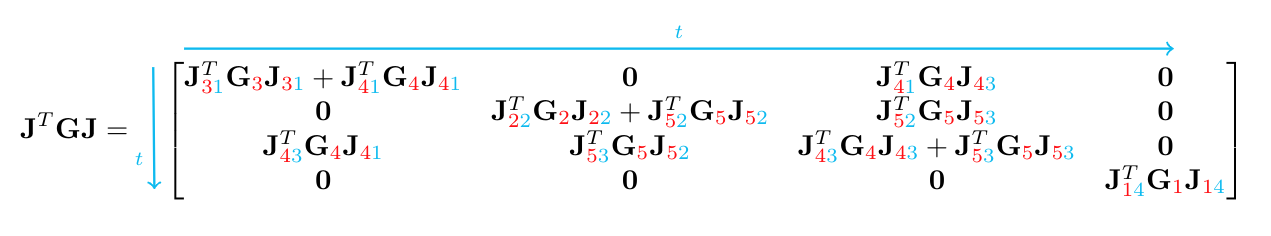
\includegraphics[width=0.8\textwidth]{figures/JTGJ_schematic.png}
	\caption{\label{fig:JTGJ_schematic} 
	Block sparsity of the $\mf{J}^T\mf{G}\mf{J}$ for the example illustrated in
	Fig. \ref{fig:sparsity_example}.}
\end{figure*}

Our implementation organizes the blocks of the Jacobian $\mf{J}$ as described in
this section, i.e. we condense rows by patches and columns by trees, so that the
supernodal Cholesky factorization can exploit this rich structure. Using this
block structure, the supernodal solver can take full advantage of specific
optimizations for dense algebra.



\subsection{Stopping Criteria}
\label{sec:stopping_criteria}

To assess convergence, we monitor the optimality condition for the unconstrained
problem in Eq. (\ref{eq:primal_unconstrained}) by evaluating the norm of the
momentum balance in Eq. (\ref{eq:primal_gradient})
\begin{equation}
	\nabla\ell_p(\mf{v}) = \mf{A}(\mf{v}-\mf{v}^*) - \mf{J}^T\bgamma.
\end{equation}

Notice that the components of $\nabla\ell_p$ have units of generalized momentum
$\mf{p}=\mf{M}\mf{v}$. Depending on the choice of generalized coordinates, the
generalized momentum components may have different units. In order to weigh all
components equally, we define the diagonal matrix $\mf{D} =
\text{diag}(\mf{M})^{-1/2}$ and perform the following change of variables
\begin{align}
	\tilde{\nabla}\ell_p &= \mf{D}\nabla\ell_p, \nonumber\\
	\tilde{\mf{p}} &= \mf{D}\mf{p}, \nonumber \\
	\tilde{\mf{j}}_c &= \mf{D}\mf{j}_c,
	\label{eq:scaled_momentum_quantities}
\end{align}
where we define the generalized contact impulse $\mf{j}_c=\mf{J}^T\bgamma$.
With this scaling, all the new \emph{tilde} variables have the same units,
square root of Joules. Using these definitions, we write our stopping criteria
as
\begin{equation}
	\Vert\tilde{\nabla}\ell_p\Vert < \varepsilon_a + \varepsilon_r\max(\Vert\tilde{\mf{p}}\Vert,\Vert\tilde{\mf{j}_c}\Vert).
	\label{eq:stopping_criteria}
\end{equation}
where $\varepsilon_r$ is a dimensionless relative tolerance that we usually set
in the range from $10^{-6}$ to $10^{-3}$. The absolute tolerance $\varepsilon_a$
is used to detect rare cases where the solution leads to no contact and no
motion, typically due to external forces. We always set this tolerance to a
small number, $\varepsilon_a=10^{-16}$.
